\documentclass[oneside]{book}
\usepackage[utf8]{inputenc}
\usepackage[english]{babel}
\usepackage{nameref}
\usepackage[acronym,numberedsection=nameref,toc]{glossaries}
\usepackage{multicol}
\usepackage[marginparwidth=75pt, margin=2cm]{geometry}
\usepackage{listings}
\usepackage{marginnote}
\usepackage{parskip}
\usepackage{titlesec}
\usepackage{enumitem}
\usepackage[hidelinks]{hyperref}
\usepackage{tikz}
\usetikzlibrary{arrows,automata,positioning}

\titleformat{\chapter}
  {\LARGE\bfseries}{\thechapter}{10pt}{}
\titlespacing{\chapter}{0pt}{0pt}{10pt}

\renewcommand{\familydefault}{\sfdefault}

\setcounter{secnumdepth}{3} % number subsections
\newcommand{\Ch}[2]{\chapter[#1]{#1\hfill[#2]}\label{#2}}
\newcommand{\Sec}[2]{\section[#1]{#1\hfill[#2]}\label{#2}}
\newcommand{\Sub}[2]{\subsection[#1]{#1\hfill[#2]}\label{#2}}
\newcommand{\SubSub}[2]{\subsubsection[#1]{#1\hfill[#2]}\label{#2}}

\makeglossaries

\newacronym{hlsl}{HLSL}{High Level Shader Language}
\newacronym{dxc}{DXC}{DirectX Shader Compiler}
\newacronym{fxc}{FXC}{Legacy DirectX Shader Compiler}
\newacronym{c}{C}{C Programming Language}
\newacronym{cpp}{C++}{C++ Programming Language}
\newacronym{api}{API}{Application Programming Interface}
\newacronym{spmd}{SPMD}{Single Program Multiple Data}
\newacronym{simd}{SIMD}{Single Instruction Multiple Data}

\newglossaryentry{spirv}
{
  name={SPIR-V},
  description={SPIR-V is a portable intermediate representation designed by the
  Khronos Group for representing GPU programs}
}

\newglossaryentry{dx}
{
  name={DirectX},
  description={DirectX is the multimedia \acrshort{api} introduced with Windows
  95.}
}

\newglossaryentry{isoC}
{
  name={ISO/IEC 9899:2018},
  description={ISO C standard}
}

\newglossaryentry{isoCPP}
{
  name={ISO/IEC 14882:2020},
  description={ISO C++ standard}
}

\newglossaryentry{sm}
{
  name={Shader Model},
  description={Versioned hardware description included as part of the DirectX
  specification, which is used for code generation of GPU code to a common set
  of features across a range of vendors.}
}

\newglossaryentry{lane}{
  name={Lane},
  description={The computation performed on a single element as described in the
  \acrshort{spmd} program. Also called: thread.}
}

\newglossaryentry{wave}{
  name={Wave},
  description={A group of \gls{lane}s which execute together. The number of
  \gls{lane}s in a Wave varies by hardware implementation. Also called: warp,
  SIMD-group, subgroup, or wavefront.}
}

\newglossaryentry{quad}{
  name={Quad},
  description={A group of four \gls{lane}s which form a cluster of adjacent
  computations in the data topology. Also called: quad-group or quad-wave. }
}

\newglossaryentry{threadgroup}{
  name={Thread Group},
  description={A group of one or more \gls{wave}s which comprise a larger
  computation. Also known as: group, workgroup, block or thread block.}
}

\newglossaryentry{dispatch}{
  name={Dispatch},
  description={A group of one or more \gls{threadgroup}s which comprise the
  largest unit of a shader execution. Also called: grid, compute space or index
  space.}
}


\title{High-Level Shader Language Specification\\
       \normalsize{Working Draft}}


\newenvironment{note}
    {\begin{center}
    \begin{tabular}{|p{0.9\textwidth}|}
    \hline\\
    }
    {
    \\\\\hline
    \end{tabular}
    \end{center}
    }

\usepackage{titleps}
\newpagestyle{body}{
  \sethead{}{}{\sectiontitle}
  \setfoot{}{}{Working Draft}
}
\pagestyle{body}

\setcounter{secnumdepth}{3}
\newcommand{\parnum}{\textbf{\arabic{parcount}}}

\setlength\parindent{0cm}

\newcommand{\newparcounter}[1]{
\newcounter{#1}
\counterwithin{#1}{chapter}
\counterwithin{#1}{section}
\counterwithin{#1}{subsection}
\counterwithin{#1}{subsubsection}
}

\newparcounter{parcount}
\newcommand\p{%
    \stepcounter{parcount}%
    \parnum \hspace{1em}%
}

\newenvironment{parnumbers}{%
   \par%
   \everypar{\noindent \stepcounter{parcount}\parnum \hspace{1em}}%
}{}

\newcommand{\Par}[2]{\paragraph[#1]{#1\hfill[#2]\\}\label{#2}\p}

\begin{document}
%%------------------------------------------------------------------------------
%% Grammar formatting
%%------------------------------------------------------------------------------

\newlength{\GrammarIndent}
\setlength{\GrammarIndent}{\leftmargini}
\newlength{\GrammarInc}
\setlength{\GrammarInc}{\GrammarIndent}
\newlength{\GrammarRest}
\setlength{\GrammarRest}{2\GrammarIndent}

\newenvironment{grammar} {
  \newcommand{\define}[1]{{\textit{##1}\textnormal{:}}}
  \newcommand{\terminal}[1]{{\textnormal{##1}}}
  \newcommand{\keyword}[1]{\texttt{##1}}
  \newcommand{\br}{\hfill\\*}

  \renewcommand{\texttt}[1]{{\small\ttfamily\upshape ##1}}

  \newcommand{\grammarindentfirst}{\GrammarIndent}
  \newcommand{\grammarindentinc}{\GrammarInc}
  \newcommand{\grammarindentrest}{\GrammarRest}
  \itshape

  \begin{grammarlist}
  \item\relax
}{
  \end{grammarlist}
}

\newlist{grammarlist}{itemize}{1}
\setlist[grammarlist]{
  parsep=1ex, partopsep=0pt, itemsep=0pt, topsep=0pt, label={},
  leftmargin=\grammarindentrest, listparindent=-\grammarindentinc,
  itemindent=\listparindent
}


\maketitle

\tableofcontents
\Ch{Introduction}{Intro}

\p The \acrfull{hlsl} is the GPU programming language provided in conjunction
with the \gls{dx} runtime. Over many years its use has expanded to cover every
major rendering API across all major development platforms. Despite its
popularity and long history \acrshort{hlsl} has never had a formal language
specification. This document seeks to change that.

\p \acrshort{hlsl} draws heavy inspiration originally from \gls{isoC} and later
from \gls{isoCPP} with additions specific to graphics and parallel computation
programming. The language is also influenced to a lesser degree by other popular
graphics and parallel programming languages.

\p \acrshort{hlsl} has two reference implementations which this specification
draws heavily from. The original reference implementation \acrfull{fxc} has been
in use since \gls{dx} 9. The more recent reference implementation \acrfull{dxc}
has been the primary shader compiler since \gls{dx} 12.

\p In writing this specification bias is leaned toward the language
behavior of \acrshort{dxc} rather than the behavior of \acrshort{fxc}, although
that can vary by context.

\p In very rare instances this spec will be aspirational, and may diverge from
both reference implementation behaviors. This will only be done in instances
where there is an intent to alter implementation behavior in the future. Since
this document and the implementations are living sources, one or the other may
be ahead in different regards at any point in time.

\Sec{Scope}{Intro.Scope}

\p This document specifies the requirements for implementations of
\acrshort{hlsl}. The \acrshort{hlsl} specification is based on and highly
influenced by the specifications for the \acrfull{c} and the \acrfull{cpp}.

\p This document covers both describing the language grammar and semantics for
\acrshort{hlsl}, and (in later sections) the standard library of data types used
in shader programming.

\Sec{Normative References}{Intro.Refs}

\p The following referenced documents provide significant influence on this
document and should be used in conjunction with interpreting this standard.

\begin{itemize}
  \item \gls{isoC}, \textit{Programming languages - C}
  \item \gls{isoCPP}, \textit{Programming languages - C++}
  \item \gls{dx} Specifications, \textit{https://microsoft.github.io/DirectX-Specs/}
\end{itemize}

\Sec{Terms and definitions}{Intro.Terms}

\p This document aims to use terms consistent with their definitions in
\gls{isoC} and \gls{isoCPP}. In cases where the definitions are unclear, or
where this document diverges from \gls{isoC} and \gls{isoCPP}, the definitions
in this section, the remaining sections in this chapter, and the attached
glossary (\ref{main}) supersede other sources.

\Sec{Common Definitions}{Intro.Defs}

\p The following definitions are consistent between \acrshort{hlsl} and the
\gls{isoC} and \gls{isoCPP} specifications, however they are included here for
reader convenience.

\Sub{Correct Data}{Intro.Defs.CorrectData}
\p Data is correct if it represents values that have specified or unspecified
but not undefined behavior for all the operations in which it is used. Data that
is the result of undefined behavior is not correct, and may be treated as
undefined.

\Sub{Diagnostic Message}{Intro.Defs.Diags}
\p An implementation defined message belonging to a subset of the
implementation's output messages which communicates diagnostic information to
the user.

\Sub{Ill-formed Program}{Intro.Defs.IllFormed}
\p A program that is not well-formed, for which the implementation is expected
to return unsuccessfully and produce one or more diagnostic messages.

\Sub{Implementation-defined Behavior}{Intro.Defs.ImpDef}
\p Behavior of a well-formed program and correct data which may vary by the
implementation, and the implementation is expected to document the behavior.

\Sub{Implementation Limits}{Intro.Defs.ImpLimits}
\p Restrictions imposed upon programs by the implementation of either the
compiler or runtime environment. The compiler may seek to surface
runtime-imposed limits to the user for improved user experience.

\Sub{Undefined Behavior}{Intro.Defs.Undefined}
\p Behavior of invalid program constructs or incorrect data for which this
standard imposes no requirements, or does not sufficiently detail.

\Sub{Unspecified Behavior}{Intro.Defs.Unspecified}
\p Behavior of a well-formed program and correct data which may vary by the
implementation, and the implementation is not expected to document the behavior.

\Sub{Well-formed Program}{Intro.Defs.WellFormed}
\p An \acrshort{hlsl} program constructed according to the syntax rules,
diagnosable semantic rules, and the One Definition Rule.

\Sub{Runtime Implementation}{Intro.Defs.Runtime}
\p A runtime implementation
refers to a full-stack implementation of a software runtime that can facilitate
the execution of \acrshort{hlsl} programs. This broad definition includes
libraries and device driver implementations. The \acrshort{hlsl} specification
does not distinguish between the user-facing programming interfaces and the
vendor-specific backing implementation.

\Sec{Runtime Targeting}{Intro.Runtime}

\p \acrshort{hlsl} emerged from the evolution of \gls{dx} to grant greater
control over GPU geometry and color processing. It gained popularity because it
targeted a common hardware description which all conforming drivers were
required to support. This common hardware description, called a \gls{sm}, is an
integral part of the description for \acrshort{hlsl} . Some \acrshort{hlsl}
features require specific \gls{sm} features, and are only supported by compilers
when targeting those \gls{sm} versions or later.

\Sec{\acrlong{spmd} Programming Model}{Intro.Model}

\p \acrshort{hlsl} uses a \acrfull{spmd} programming model where a program
describes operations on a single element of data, but when the program executes
it executes across more than one element at a time. This programming model is
useful due to GPUs largely being \acrfull{simd} hardware architectures where
each instruction natively executes across multiple data elements at the same
time.

\p There are many different terms of art for describing the elements of a GPU
architecture and the way they relate to the \acrshort{spmd} program model. In
this document we will use the terms as defined in the following subsections.

\Sub{\acrshort{spmd} Terminology}{Intro.Model.Terms}

\SubSub{Host and Device}{Intro.Model.Terms.HostDevice}

\p \acrshort{hlsl} is a data-parallel programming language designed for
programming auxiliary processors in a larger system. In this context the
\textit{host} refers to the primary processing unit that runs the application
which in turn uses a runtime to execute \acrshort{hlsl} programs on a supported
\textit{device}. There is no strict requirement that the host and device be
different physical hardware, although they commonly are. The separation of host
and device in this specification is useful for defining the execution and memory
model as well as specific semantics of language constructs.

\SubSub{\gls{lane}}{Intro.Model.Terms.Lane}

\p A \gls{lane} represents a single computed element in an \acrshort{spmd}
program. In a traditional programming model it would be analogous to a thread of
execution, however it differs in one key way. In multi-threaded programming
threads advance independent of each other. In \acrshort{spmd} programs, a group
of \gls{lane}s may execute instructions in lockstep because each instruction may
be a \acrshort{simd} instruction computing the results for multiple \gls{lane}s
simultaneously, or synchronizing execution across multiple \gls{lane}s or
\gls{wave}s. A \gls{lane} has an associated \textit{lane state} which denotes
the execution status of the lane (\ref{Intro.Model.Terms.LaneState}).

\SubSub{\gls{wave}}{Intro.Model.Terms.Wave}

\p A grouping of \gls{lane}s for execution is called a \gls{wave}. The size of a
\gls{wave} is defined as the maximum number of \textit{active} \gls{lane}s the
\gls{wave} supports. \gls{wave} sizes vary by hardware architecture, and are required
to be powers of two. The number of \textit{active} \gls{lane}s in a \gls{wave}
can be any value between one and the \gls{wave} size.

\p Some hardware implementations support multiple \gls{wave} sizes. There is no
overall minimum wave size requirement, although some language features do have
minimum \gls{lane} size requirements.

\p \acrshort{hlsl} is explicitly designed to run on hardware with arbitrary
\gls{wave} sizes. Hardware architectures may implement \gls{wave}s as
\acrfull{simt} where each thread executes instructions in lockstep. This is not
a requirement of the model. Some constructs in \acrshort{hlsl} require
synchronized execution. Such constructs will explicitly specify that
requirement.

\SubSub{\gls{quad}}{Intro.Model.Terms.Quad}

\p A \gls{quad} is a subdivision of four \gls{lane}s in a \gls{wave} which are
computing adjacent values. In pixel shaders a \gls{quad} may represent four
adjacent pixels and \gls{quad} operations allow passing data between adjacent
\gls{lane}s. In compute shaders quads may be one or two dimensional depending
on the workload dimensionality. Quad operations require four active \gls{lane}s.

\SubSub{\gls{threadgroup}}{Intro.Model.Terms.Group}

\p A grouping of \gls{lane}s executing the same shader to produce a combined
result is called a \gls{threadgroup}. \gls{threadgroup}s are independent of
\acrshort{simd} hardware specifications. The dimensions of a \gls{threadgroup}
are defined in three dimensions. The maximum extent along each dimension of a
\gls{threadgroup}, and the total size of a \gls{threadgroup} are implementation
limits defined by the runtime and enforced by the compiler. If a
\gls{threadgroup}'s size is not a whole multiple of the hardware \gls{wave}
size, the unused hardware \gls{lane}s are implicitly inactive.

\p If a \gls{threadgroup} size is smaller than the \gls{wave} size , or if the
\gls{threadgroup} size is not an even multiple of the \gls{wave} size, the
remaining \gls{lane} are \textit{inactive} \gls{lane}s.

\SubSub{\gls{dispatch}}{Intro.Model.Terms.Dispatch}

\p A grouping of \gls{threadgroup}s which represents the full execution of a
\acrshort{hlsl} program and results in a completed result for all input data
elements.

\SubSub{\gls{lane} States}{Intro.Model.Terms.LaneState}

\p \gls{lane}s may be in three primary states: \textit{active}, \textit{helper},
\textit{inactive}, and \textit{predicated off}.

\p An \textit{active} \gls{lane} is enabled to perform computations and produce
output results based on the initial launch conditions and program control flow.

\p A \textit{helper} \gls{lane} is a lane which would not be executed by the
initial launch conditions except that its computations are required for adjacent
pixel operations in pixel fragment shaders. A \textit{helper} \gls{lane} will
execute all computations but will not perform writes to buffers, and any outputs
it produces are discarded. \textit{Helper} lanes may be required for
\gls{lane}-cooperative operations to execute correctly.

\p A \textit{inactive} \gls{lane} is a lane that is not executed by the initial
launch conditions. This occurs when there is not sufficient inputs to fill the
all \gls{lane}s in the \gls{wave}.

\p A \textit{predicated off} \gls{lane} is a lane that is not being executed due
to program control flow. A \gls{lane} may be \textit{predicated off} when
control flow for the \gls{lane}s in a \gls{wave} diverge and one or more lanes
are temporarily not executing.

\p The diagram blow illustrates the state transitions between \gls{lane} states:

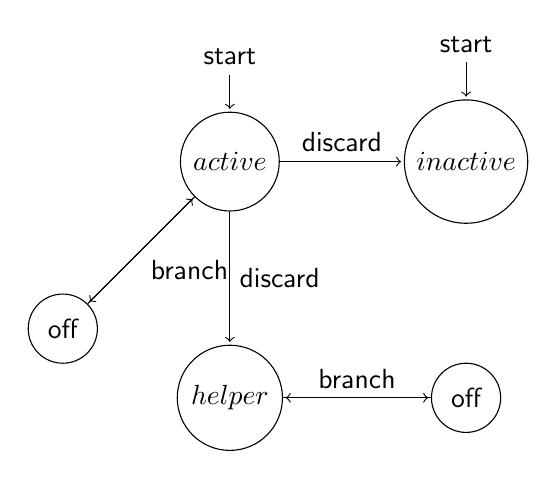
\begin{tikzpicture}[shorten >=1pt,node distance=3cm,auto, squarednode/.style={rectangle,minimum size=7mm}]
  \node[squarednode,state,initial above] (active) {$active$};
  \node[squarednode,state,initial above] (inactive)[right of=active] {$inactive$};
  \node[squarednode,state] (helper)[below of=active] {$helper$};
  \node[squarednode,state] (off1)[below left of=active] {off};
  \node[squarednode,state] (off2)[right of=helper] {off};


  \path[->] (active) edge node {discard} (inactive);
  \path[->] (active) edge node {discard} (helper);
  \path[->] (active) edge node {branch} (off1);
  \path[->] (off1) edge node {} (active);

  \path[->] (helper) edge node {branch} (off2);
  \path[->] (off2) edge node {} (helper);
\end{tikzpicture}

\Sub{\acrshort{spmd} Execution Model}{Intro.Model.Exec}

\p A runtime implementation shall provide an implementation-defined mechanism
for defining a \gls{dispatch}. A runtime shall manage hardware resources and
schedule execution to conform to the behaviors defined in this specification in
an implementation-defined way. A runtime implementation may sort the
\gls{threadgroup}s of a \gls{dispatch} into \gls{wave}s in an
implementation-defined way. During execution no guarantees are made that all
\gls{lane}s in a \gls{wave} are actively executing.

\p \gls{wave}, \gls{quad}, and \gls{threadgroup} operations require execution
synchronization of applicable active and helper \gls{lane}s as defined by the
individual operation.

\Sub{Optimization Restrictions}{Intro.Model.Restrictions}

\p An optimizing compiler may not optimize code generation such that it changes
the behavior of a well-formed program except in the presence of
\textit{implementation-defined} or \textit{unspecified} behavior.

\p The presence of \gls{wave}, \gls{quad}, or \gls{threadgroup} operations
may further limit the valid transformations of a program. Specifically, control
flow operations which result in changing which \gls{lane}s, \gls{quad}s, or
\gls{wave}s are actively executing are illegal in the presence of cooperative
operations if the optimization alters the behavior of the program.

\Sec{\acrshort{hlsl} Memory Models}{Intro.Memory}

\p Memory accesses for \gls{sm} 5.0 and earlier operate on 128-bit slots aligned
on 128-bit boundaries. This optimized for the common case in early shaders where
data being processed on the GPU was usually 4-element vectors of 32-bit data
types.

\p On modern hardware memory access restrictions are loosened, and reads of
32-bit multiples are supported starting with \gls{sm} 5.1 and reads of 16-bit
multiples are supported with \gls{sm} 6.0. \gls{sm} features are fully
documented in the \gls{dx} Specifications, and this document will not attempt to
elaborate further.

\Sub{Memory Spaces}{Intro.Memory.Spaces}

\p \acrshort{hlsl} programs manipulate data stored in four distinct memory
spaces: thread, threadgroup, device and constant.

\SubSub{Thread Memory}{Intro.Memory.Spaces.Thread}

\p Thread memory is local to the \gls{lane}. It is the default memory space used to
store local variables. Thread memory cannot be directly read from other threads
without the use of intrinsics to synchronize execution and memory.

\SubSub{\gls{threadgroup} Memory}{Intro.Memory.Spaces.Group}

\p \gls{threadgroup} memory is denoted in \acrshort{hlsl} with the
\texttt{groupshared} keyword. The underlying memory for any declaration
annotated with \texttt{groupshared} is shared across an entire
\gls{threadgroup}. Reads and writes to \gls{threadgroup} Memory, may occur in
any order except as restricted by synchronization intrinsics or other memory
annotations.

\SubSub{Device Memory}{Intro.Memory.Spaces.Device}

\p Device memory is memory available to all \gls{lane}s executing on the device.
This memory may be read or written to by multiple \gls{threadgroup}s that are
executing concurrently. Reads and writes to device memory may occur in any order
except as restricted by synchronization intrinsics or other memory annotations.
Some device memory may be visible to the host. Device memory that is visible to
the host may have additional synchronization concerns for host visibility.

\SubSub{Constant Memory}{Intro.Memory.Spaces.Constant}

\p Constant memory is similar to device memory in that it is available to all
\gls{lane}s executing on the device. Constant memory is read-only, and an
implementation can assume that constant memory is immutable and cannot change
during execution.

\Ch{Lexical Conventions}{Lex}

\Sec{Unit of Translation}{Lex.Translation}

\p The text of \acrshort{hlsl} programs is collected in \textit{source} and
\textit{header} files. The distinction between source and header files is social
and not technical. An implementation will construct a \textit{translation unit}
from a single source file and any included source or header files referenced via
the \texttt{\#include} preprocessing directive conforming to the \gls{isoC}
preprocessor specification.

\p An implementation may implicitly include additional sources as required to
expose the \acrshort{hlsl} library functionality as defined in (\ref{Runtime}).

\Sec{Phases of Translation}{Lex.Phases}

\p \acrshort{hlsl} inherits the phases of translation from \gls{isoCPP}, with
minor alterations, specifically the removal of support for trigraph and digraph
sequences. Below is a description of the phases.

\begin{enumerate}
  \item Source files are characters that are mapped to the basic source
  character set in an implementation-defined manner.
  \item Any sequence of backslash (\texttt{\textbackslash}) immediately followed
  by a new line is deleted, resulting in splicing lines together.
  \item Tokenization occurs and comments are isolated. If a source file ends in
  a partial comment or preprocessor token the program is ill-formed and a
  diagnostic shall be issued. Each comment block shall be treated as a single
  white-space character.
  \item Preprocessing directives are executed, macros are expanded,
  \texttt{pragma} and other unary operator expressions are executed. Processing
  of \texttt{\#include} directives results in all preceding steps being executed
  on the resolved file, and can continue recursively. Finally all preprocessing
  directives are removed from the source.
  \item Character and string literal specifiers are converted into the
  appropriate character set for the execution environment.
  \item Adjacent string literal tokens are concatenated.
  \item White-space is no longer significant. Syntactic and semantic analysis
  occurs translating the whole translation unit into an implementation-defined
  representation.
  \item The translation unit is processed to determine required instantiations,
  the definitions of the required instantiations are located, and the
  translation and instantiation units are merged. The program is ill-formed if
  any required instantiation cannot be located or fails during instantiation.
  \item External references are resolved, library references linked, and all
  translation output is collected into a single output.
\end{enumerate}

\Sec{Character Sets}{Lex.CharSet}

\p The \textit{basic source character set} is a subset of the ASCII character set.
The table below lists the valid characters and their ASCII values:

\begin{center}
  \begin{tabular}{|| c | c | c ||}
    \hline
    Hex ASCII Value & Character Name & Glyph or C Escape Sequence \\
    \hline
    0x09 & Horizontal Tab & \texttt{\textbackslash t} \\
    0x0A & Line Feed & \texttt{\textbackslash n} \\
    0x0D & Carriage Return & \texttt{\textbackslash r} \\
    0x20 & Space & \\
    0x21 & Exclamation Mark & \texttt{!}\\
    0x22 & Quotation Mark & \texttt{"}\\
    0x23 & Number Sign & \texttt{\#}\\
    0x25 & Percent Sign & \texttt{\%}\\
    0x26 & Ampersand & \texttt{\&}\\
    0x27 & Apostrophe & \texttt{'}\\
    0x28 & Left Parenthesis & \texttt{(}\\
    0x29 & Right Parenthesis & \texttt{)}\\
    0x2A & Asterisk & \texttt{*}\\
    0x2B & Plus Sign & \texttt{+}\\
    0x2C & Comma & \texttt{,}\\
    0x2D & Hyphen-Minus & \texttt{-}\\
    0x2E & Full Stop & \texttt{.}\\
    0x2F & Solidus & \texttt{/}\\
    0x30 .. 0x39 & Digit Zero .. Nine & \texttt{0 1 2 3 4 5 6 7 8 9}\\
    0x3A & Colon & \texttt{:}\\
    0x3B & Semicolon & \texttt{;}\\
    0x3C & Less-than Sign & \texttt{<}\\
    0x3D & Equals Sign & \texttt{=}\\
    0x3E & Greater-than Sign & \texttt{>}\\
    0x3F & Question Mark & \texttt{?}\\
    0x41 .. 0x5A & Latin Capital Letter A .. Z &
        \texttt{A B C D E F G H I J K L M}\\
    & & \texttt{N O P Q R S T U V W X Y Z}\\
    0x5B & Left Square Bracket & \texttt{[}\\
    0x5C & Reverse Solidus & \texttt{\textbackslash}\\
    0x5D & Right Square Bracket & \texttt{[}\\
    0x5E & Circumflex Accent & \texttt{\textasciicircum}\\
    0x5F & Underscore & \texttt{\_}\\
    0x61 .. 0x7A & Latin Small Letter a .. z &
        \texttt{a b c d e f g h i j k l m}\\
    & & \texttt{n o p q r s t u v w x y z}\\
    0x7B & Left Curly Bracket & \texttt{\{}\\
    0x7C & Vertical Line & \texttt{|}\\
    0x7D & Right Curly Bracket & \texttt{\}}\\
    \hline
  \end{tabular}
\end{center}

\p An implementation may allow source files to be written in alternate
\textit{extended character sets} as long as that set is a superset of the
\textit{basic character set}. The \textit{translation character set} is an
\textit{extended character set} or the \textit{basic character set} as chosen by
the implementation.

\Sec{Preprocessing Tokens}{Lex.PPTokens}

\begin{grammar}
  \define{preprocessing-token}\br
  header-name\br
  identifier\br
  pp-number\br
  character-literal\br
  string-literal\br
  preprocessing-op-or-punc\br
  \textnormal{each non-whitespace character from the \textit{translation
  character set} that cannot be one of the above}
\end{grammar}\footnote{The preprocessor is inherited from C++ 11 with no
grammar extensions. It is specified here only for completeness.}

\p Each preprocessing token that is converted to a token shall have the lexical
form of a keyword, an identifier, a constant, a string literal or an operator or
punctuator.

\p Preprocessing tokens are the minimal lexical elements of the language during
translation phases 3 through 6 (\ref{Lex.Phases}). Preprocessing tokens can be
separated by whitespace in the form of comments, white space characters, or
both. White space may appear within a preprocessing token only as part of a
header name or between the quotation characters in a character constant or
string literal.

\p Header name preprocessing tokens are only recognized within
\texttt{\#include} preprocessing directives, \texttt{\_\_has\_include} expressions,
and implementation-defined locations within \texttt{\#pragma} directives. In
those contexts, a sequence of characters that could be either a header name or a
string literal is recognized as a header name.

\Sec{Tokens}{Lex.Tokens}

\begin{grammar}
  \define{token}\br
  identifier\br
  keyword\br
  literal\br
  operator-or-punctuator
\end{grammar}

\p There are five kinds of tokens: identifiers, keywords, literals, and
operators or punctuators. All whitespace characters and comments are ignored
except as they separate tokens.

\Sec{Comments}{Lex.Comments}

\p The characters \texttt{/*} start a comment which terminates with the
characters \texttt{*/}. The characters \texttt{//} start a comment
which terminates at the next new line.

\Sec{Header Names}{Lex.Headers}

\begin{grammar}
  \define{header-name}\br
  \texttt{<} h-char-sequence \texttt{>}\br
  \texttt{"} q-char-sequence \texttt{"}

  \define{h-char-sequence}\br
  h-char\br
  h-char-sequence h-char

  \define{h-char}\br
  \textnormal{any character in the \textit{translation character set} except
  newline or \texttt{>}}

  \define{q-char-sequence}\br
  q-char\br
  q-char-sequence q-char

  \define{q-char}\br
  \textnormal{any character in the \textit{translation character set} except
  newline or \texttt{"}}
\end{grammar}

\p Character sequences in header names are mapped to header files or external
source file names in an implementation defined way.

\Sec{Preprocessing numbers}{Lex.PPNumber}

\begin{grammar}
  \define{pp-number}\br
  digit\br
  \texttt{.} digit\br
  pp-number \texttt{'} digit\br
  pp-number \texttt{'} non-digit\br
  pp-number \texttt{e} sign\br
  pp-number \texttt{E} sign\br
  pp-number \texttt{p} sign\br
  pp-number \texttt{P} sign\br
  pp-number \texttt{.}
\end{grammar}

\p Preprocessing numbers begin with a digit or period (\texttt{.}), and may be
followed by valid identifier characters and floating point literal suffixes
(\texttt{e+}, \texttt{e-}, \texttt{E+}, \texttt{E-}, \texttt{p+}, \texttt{p-},
\texttt{P+}, and \texttt{P-}). Preprocessing number tokens lexically include all
\textit{integer-literal} and \textit{floating-literal} tokens.

\p Preprocessing numbers do not have types or values. Types and values are
assigned to \textit{integer-literal}, \textit{floating-literal}, and
\textit{vector-literal} tokens on successful conversion from preprocessing
numbers.

\p A preprocessing number cannot end in a period (\texttt{.}) if the immediate
next token is a \textit{scalar-element-sequence} (\ref{Lex.Literal.Vector}). In
this situation the \textit{pp-number} token is truncated to end before the
period\footnote{This grammar formulation is not context-free and requires an
LL(2) parser.}.

%\Sec{Identifiers}{Lex.Ident}

%\Sec{Keywords}{Lex.Keywords}

%\Sec{Operators and Punctuators}{Lex.Operators}

\Sec{Literals}{Lex.Literals}

\Sub{Literal Classifications}{Lex.Literal.Kinds}

\begin{grammar}
  \define{literal}\br
  integer-literal\br
  character-literal\br
  floating-literal\br
  string-literal\br
  boolean-literal\br
  vector-literal
\end{grammar}

\Sub{Integer Literals}{Lex.Literal.Int}

\begin{grammar}
  \define{integer-literal}\br
  decimal-literal \opt{integer-suffix}\br
  octal-literal \opt{integer-suffix}\br
  hexadecimal-literal \opt{integer-suffix}\br

  \define{decimal-literal}\br
  nonzero-digit\br
  decimal-literal digit\br

  \define{octal-literal}
  \terminal{0}\br
  octal-literal octal-digit\br

  \define{hexadecimal-literal}\br
  \terminal{0x} hexadecimal-digit\br
  \terminal{0X} hexadecimal-digit\br
  hexadecimal-literal hexadecimal-digit\br

  \define{nonzero-digit} \textnormal{one of}\br
  \terminal{1 2 3 4 5 6 7 8 9}\br

  \define{octal-digit} \textnormal{one of}\br
  \terminal{0 1 2 3 4 5 6 7}\br

  \define{hexadecimal-digit} \textnormal{one of}\br
  \terminal{0 1 2 3 4 5 6 7 8 9}\br
  \terminal{a b c d e f}\br
  \terminal{A B C D E F}\br

  \define{integer-suffix}\br
  unsigned-suffix \opt{long-suffix}\br
  long-suffix \opt{unsigned-suffix}\br

  \define{unsigned-suffix} \textnormal{one of}\br
  \terminal{u U}\br

  \define{long-suffix} \textnormal{one of}\br
  \terminal{l L}
\end{grammar}

\p An \textit{integer literal} is an optional base prefix, a sequence of digits
in the appropriate base, and an optional type suffix. An integer literal shall
not contain a period or exponent specifier.

\p The type of an integer literal is the first of the corresponding list in the
table below in which its value can be represented\footnote{This behavior matches
\gls{isoC} but is reduced in scope because HLSL has fewer data types.}.

\begin{center}
  \begin{tabular}{|| c | c | c ||}
    \hline
    Suffix & Decimal constant & Octal or hexadecimal constant \\
    \hline
    \hline
    none & \texttt{int32\_t} & \texttt{int32\_t} \\
         & \texttt{int64\_t} & \texttt{uint32\_t} \\
         &         & \texttt{int64\_t} \\
         &         & \texttt{uint64\_t} \\
    \hline
    \texttt{u} or \texttt{U} & \texttt{uint32\_t} & \texttt{uint32\_t} \\
                             & \texttt{uint64\_t} & \texttt{uint64\_t} \\
    \hline
    \texttt{l} or \texttt{L} & \texttt{int64\_t} & \texttt{int64\_t} \\
                             &  & \texttt{uint64\_t} \\
    \hline
    Both \texttt{u} or \texttt{U} & \texttt{uint64\_t} & \texttt{uint64\_t} \\
    and \texttt{l} or \texttt{L}  &  &  \\
    \hline
  \end{tabular}
\end{center}

\p If the specified value of an integer literal cannot be represented by any
type in the corresponding list, the integer literal has no type and the program
is ill-formed.

\p An implementation may support the integer suffixes \texttt{ll} and
\texttt{ull} as equivalent to \texttt{l} and \texttt{ul} respectively.

%\Sub{Character Literals}{Lex.Literal.Char}

\Sub{Floating-point Literals}{Lex.Literal.Float}

\begin{grammar}
  \define{floating-literal}\br
  fractional-constant \opt{exponent-part} \opt{floating-suffix}\br
  digit-sequence exponent-part \opt{floating-suffx}\br
  \define{fractional-constant}\br
  \opt{digit-sequence} \texttt{.} digit-sequence\br
  digit-sequence \texttt{.}\br
  \define{exponent-part}\br
  \texttt{e} \opt{sign} digit-sequence\br
  \texttt{E} \opt{sign} digit-sequence\br
  \define{sign} \textnormal{one of}\br
  \texttt{+} \texttt{-}\br
  \define{digit-sequence}\br
  digit\br
  digit-sequence digit
  \define{floating-suffix} \textnormal{one of}
  \texttt{h} \texttt{f} \texttt{l} \texttt{H} \texttt{F} \texttt{L}
\end{grammar}

\p A floating literal is written either as a \textit{fractional-constant} with
an optional \textit{exponent-part} and optional \textit{floating-suffix}, or as
an integer \textit{digit-sequence} with a required \textit{exponent-part} and
optional \textit{floating-suffix}.

\p The type of a floating literal is \texttt{float}, unless explicitly specified
by a suffix. The suffixes \texttt{h} and \texttt{H} specify \texttt{half}, the
suffixes \texttt{f} and \texttt{F} specify \texttt{float}, and the suffixes
\texttt{l} and \texttt{L} specify \texttt{double}.\footnote{This substantially
deviates from the implementations in \acrshort{fxc} and \acrshort{dxc}, but is
consistent with the
\href{https://learn.microsoft.com/en-us/windows/win32/direct3dhlsl/dx-graphics-hlsl-appendix-grammar\#floating-point-numbers}
{official documentation} and the behavior of GLSL. It is also
substantially simpler to implement and more regular than the existing
behaviors.} If a value specified in the source is not in the range of
representable values for its type, the program is ill-formed.

%\Sub{String Literals}{Lex.Literal.String}

%\Sub{Boolean Literals}{Lex.Literal.Bool}

\Sub{Vector Literals}{Lex.Literal.Vector}

\begin{grammar}
  \define{vector-literal}\br
  integer-literal \texttt{.} scalar-element-sequence\br
  floating-literal \texttt{.} scalar-element-sequence

  \define{scalar-element-sequence}\br
  scalar-element-sequence-x\br
  scalar-element-sequence-r

  \define{scalar-element-sequence-x}\br
  \texttt{x}\br
  scalar-element-sequence-x \texttt{x}

  \define{scalar-element-sequence-r}\br
  \texttt{r}\br
  scalar-element-sequence-r \texttt{r}
\end{grammar}

\p A \textit{vector-literal} is an \textit{integer-literal} or
\textit{floating-point} literal followed by a period (\texttt{.}) and a
\textit{scalar-element-sequence}.

\p A \textit{scalar-element-sequence} is a \textit{vector-swizzle-sequence}
where only the first vector element accessor is valid (\texttt{x} or
\texttt{r}). A \textit{scalar-element-sequence} is equivalent to a vector splat
conversion performed on the \textit{integer-literal} or
\textit{floating-literal} value (\ref{Conv.vsplat}).


\Ch{Basic Concepts}{Basic}

\begin{note}
  \p HLSL inherits a significant portion of its language semantics from C and C++.
  Some of this is a result of intentional adoption of syntax early in the development
  of the language and some a side-effect of the Clang-based implementation of DXC.

  \p This chapter includes a lot of definitions that are inherited from C and C++.
  Some are identical to C or C++, others are slightly different. HLSL is neither
  a subset nor a superset of C or C++, and cannot be simply described in terms
  of C or C++. This specification includes all necessary definitions for clarity.
\end{note}

\Sec{Preamble}{Basic.preamble}

\p An \textit{entity} is a value, object, function, enumerator, type, class
member, bit-field, template, template specialization, namespace, or pack.

\p A \textit{name} is a use of an \textit{identifier} (\ref{Expr.Primary.ID}),
\textit{operator-function-id} (\ref{Overload.operator}),
\textit{conversion-function-id} (\ref{Classes.Conversions}),
or \textit{template-id} (\ref{Template}) that denotes any entity or
\textit{label} (\ref{Stmt.Label}).

\p Every name that denotes an entity is introduced by a \textit{declaration}.
Every name that denotes a label is introduced by a \textit{labeled statement}
(\ref{Stmt.Label})\footnote{HLSL does not have \texttt{goto}, and labeled
statements are only valid within \texttt{switch} statements.}.

\p A \textit{variable} is introduced by the declaration of a reference other
than a non-static data member of an object. The variable's name denotes the
reference or object.

\p Whenever a name is encountered it is necessary to determine if the name
denotes an entity that is a type or template. The process for determining if a
name refers to a type or template is called \textit{name lookup}.

\p Two names are the same name if:
\begin{itemize}
\item they are identifiers comprised of the same character sequence, or
\item they are operator-function-ids formed with the same operator, or
\item they are conversion-function-ids formed with the same type, or
\item they are template-ids that refer to the same class or function.
\end{itemize}

\p \begin{note}
  This section matches \gls{isoCPP} section \textbf{[basic]} except for the
  exclusion of \texttt{goto} and \textit{literal operators}.
\end{note}

\Sec{Declarations and definitions}{Basic.Decl}

\p A declaration (\ref{Decl}) may introduce one or more names into a translation
unit or redeclare names introduced by previous declarations. If a declaration
introduces names, it specifies the interpretation and attributes of these names.
A declaration may also have effects such as:
\begin{itemize}
\item verifying a static assertion (\ref{Decl}),
\item use of attributes (\ref{Decl}), and
\item controlling template instantiation (\ref{Template.Inst}).
\end{itemize}

\p A declaration is a \textit{definition} unless:
\begin{itemize}
\item it declares a function without specifying the function's body
(\ref{Decl.Function}),
\item it is a parameter declaration in a function declaration that does not
specify the function's body (\ref{Decl.Function}),
\item it is a global or namespace member declaration without the \texttt{static}
specifier\footnote{Global variable declarations are implicitly constant and
external in HLSL.},
\item it declares a static data member in a class definition,
\item it is a class name declaration,
\item it is a template parameter,
\item it is a \texttt{typedef} declaration (\ref{Decl}),
\item it is an \textit{alias-declaration} (\ref{Decl}),
\item it is a \textit{using-declaration} (\ref{Decl}),
\item it is a \textit{static\_assert-declaration} (\ref{Decl}),
\item it is an \textit{empty-declaration} (\ref{Decl}),
\item or a \textit{using-directive} (\ref{Decl}).
\end{itemize}

\p The two examples below is adapted from \gls{isoCPP} \textbf{[basic.def]}. All
but one of the following are definitions:
\begin{HLSL}
int f(int x) { return x+1; } // defines f and x
struct S {int a;int b;};     // defines S, S::a, and S::b
struct X {                   // defines X
  int x;                     // defines non-static member x
  static int y;              // declares static data member y
};
int X::y = 1;                // defines X::y
enum { up, down };           // defines up and down
namespace N {                // defines N
int d;                       // declares N::d
static int i;                // defines N::i
}
\end{HLSL}

\p All of the following are declarations:
\begin{HLSL}
int a;                       // declares a
const int c;                 // declares c
X anX;                       // declares anX
int f(int);                  // declares f
struct S;                    // declares S
typedef int Int;             // declares Int
using N::d;                  // declares d
using Float = float;         // declares Float
cbuffer CB {                 // does not declare CB
  int z;                     // declares z
}
tbuffer TB {                 // does not declare TB
  int w;                     // declares w
}
\end{HLSL}

\Sec{Types}{Basic.types}

\p The \textit{object representation} of an object of type \texttt{T} is the
sequence of \textit{N} bytes taken up by the object of type \texttt{T}, where
\textit{N} equals \texttt{sizeof(T)}\footnote{\texttt{sizeof(T)} returns the
size of the object as-if it's stored in device memory, and determining the size
if it's stored in another memory space is not possible.}. The \textit{object
representation} of an object may be different based on the \textit{memory space}
it is stored in (\ref{Intro.Memory.Spaces}).

\p The \textit{value representation} of an object is the set of bits that hold
the value of type \texttt{T}. Bits in the object representation that are not
part of the value representation are \textit{padding bits}.

\p An \textit{object type} is a type that is not a function type, not a
reference type, and not a void type.

\p A \textit{class type} is a data type declared with either the \texttt{class}
or \texttt{struct} keywords (\ref{Classes}). A class type \texttt{T} may be
declared as incomplete at one point in a translation unit via a \textit{forward
declaration}, and complete later with a full definition. The type \texttt{T} is
the same type throughout the translation unit.

\p There are special implementation-defined types such as \textit{handle types},
which fall into a category of \textit{standard intangible types}. Intangible
types are types that have no defined object representation or value
representation, as such the size is unknown at compile time.
% Note: The above definition is likely incomplete, and it is unclear if minimum
% precision types should be intangible.

\p A class type \texttt{T} is an \textit{intangible class type} if it contains
an base classes or members of intangible class type, standard intangible type,
or arrays of such types. Standard intangible types and intangible class types
are collectively called \textit{intangible types}(\ref{Intangible}).

\p An object type is an \textit{incomplete type} if the compiler lacks
sufficient information to determine the size of an object of type \texttt{T},
and it is not an intangible type. It is a \textit{complete type} if the compiler
has sufficient information to determine the size of an object of type
\texttt{T}, or if the type is known to be an intangible type. An object may not
be defined to have an \textit{incomplete} type.

\p Arithmetic types (\ref{Basic.types.arithmetic}), enumeration types, and
\textit{cv-qualified} versions of these types are collectively called
\textit{scalar types}.

\p Vectors of scalar types declared with the built-in \texttt{vector<T,N>}
template are \textit{vector types}. Vector lengths must be between 1 and 4 (i.e.
\( 1 \leq N \leq 4 \) ).

\Sub{Arithmetic Types}{Basic.types.arithmetic}

\p There are three \textit{standard signed integer types}: \texttt{int16\_t},
\texttt{int32\_t}, and \texttt{int64\_t}. Each of the signed integer types is
explicitly named for the size in bits of the type's object representation. There
is also the type alias \texttt{int} which is an alias of \texttt{int32\_t}.
There is one \textit{minimum precision signed integer type}: \texttt{min16int}.
The minimum precision signed integer type is named for the required minimum
value representation size in bits. The object representation of
\texttt{min16int} is \texttt{int}. The standard signed integer types and minimum
precision signed integer type are collectively called \textit{signed integer
types}.

\p There are three \textit{standard unsigned integer types}: \texttt{uint16\_t},
\texttt{uint32\_t}, and \texttt{uint64\_t}. Each of the unsigned integer types
is explicitly named for the size in bits of the type's object representation.
There is also the type alias \texttt{uint} which is an alias of
\texttt{uint32\_t}. There is one \textit{minimum precision unsigned integer
type}: \texttt{min16uint}. The minimum precision unsigned integer type is named
for the required minimum value representation size in bits. The object
representation of \texttt{min16uint} is \texttt{uint}. The standard unsigned
integer types and minimum precision unsigned integer type are collectively
called \textit{unsigned integer types}.

\p The minimum precision signed integer types and minimum precision unsigned
integer types are collectively called \textit{minimum precision integer types}.
The standard signed integer types and standard unsigned integer types are
collectively called \textit{standard integer types}. The signed integer types
and unsigned integer types are collectively called \textit{integer types}.
Integer types inherit the object representation of integers defined in
\glsdesc{isoC23}\footnote{C23 adopts two's compliment as the object
representation for integer types.}. Integer types shall satisfy the constraints
defined in \glsdesc{isoCPP}, section \textbf{basic.fundamental}.

\p There are three \textit{standard floating point types}: \texttt{half},
\texttt{float}, and \texttt{double}. The \texttt{float} type is a 32-bit
floating point type. The \texttt{double} type is a 64-bit floating point type.
Both the \texttt{float} and \texttt{double} types have object representations as
defined in \gls{IEEE754}. The \texttt{half} type may be either 16-bit or 32-bit
as controlled by implementation defined compiler settings. If \texttt{half} is
32-bit it will have an object representation as defined in \gls{IEEE754},
otherwise it will have an object representation matching the \textbf{binary16}
format defined in \gls{IEEE754}\footnote{IEEE-754 only defines a binary encoding
for 16-bit floating point values, it does not fully specify the behavior of such
types.}. There is one \textit{minimum precision floating point type}:
\texttt{min16float}. The minimum precision floating point type is named for the
required minimum value representation size in bits. The object representation of
\texttt{min16float} is \texttt{float}\footnote{This means when stored to memory
objects of type \texttt{min16float} are stored as \textbf{binary32} as defined
in \gls{IEEE754}.}. The standard floating point types and minimum precision
floating point type are collectively called \textit{floating point types}.

\p Integer and floating point types are collectively called \textit{arithmetic
types}.

\p The \texttt{void} type is inherited from \gls{isoCPP}, which defines it as
having an empty set of values and being an incomplete type that can never be
completed. The \texttt{void} type is used to signify the return type of a
function that returns no value. Any expression can be explicitly converted to
\texttt{void}.

\Sec{Lvalues and rvalues}{Basic.lval}

\p Expressions are classified by the type(s) of values they produce. The valid
types of values produced by expressions are:

\begin{enumerate}
  \item An \textit{lvalue} represents a function or object.
  \item An \textit{rvalue} represents a temporary object.
  \item An \textit{xvalue} (expiring value) represents an object near the end
  of its lifetime.
  \item A \textit{cxvalue} (casted expiring value) is an \textit{xvalue}
  which, on expiration, assigns its value to a bound \textit{lvalue}.
  \item A \textit{glvalue} is an \textit{lvalue}, \textit{xvalue}, or
  \textit{cxvalue}.
  \item A \textit{prvalue} is an \textit{rvalue} that is not an \textit{xvalue}.
\end{enumerate}


\Ch{Standard Conversions}{Conv}

\p \acrshort{hlsl} inherits standard conversions similar to \gls{isoCPP}. This
chapter enumerates the full set of conversions. A \textit{standard conversion
sequence} is a sequence of standard conversions in the following order:
\begin{enumerate}
  \item Zero or one conversion of either lvalue-to-rvalue, array-to-pointer or
  function-to-pointer.
  \item Zero or one conversion of either integral conversion, floating point
  conversion, floating point-integral conversion, or boolean conversion,
  derived-to-base-lvalue, vector splat, vector truncation, or flat conversion.
  \item Zero or one conversion of either component-wise integral conversion,
  component-wise floating point conversion, component-wise floating
  point-integral conversion, or component-wise boolean conversion.
  \item Zero or one qualification conversion.
\end{enumerate}

Standard conversion sequences are applied to expressions, if necessary, to
convert it to a required destination type.

\Sec{Lvalue-to-rvalue conversion}{Conv.lval}

\p A glvalue of a non-function type \texttt{T} can be converted to a prvalue.
The program is ill-formed if \texttt{T} is an incomplete type. If the glvalue
refers to an object that is not of type \texttt{T} and is not an object of a
type derived from \texttt{T}, the program is ill-formed. If the glvalue refers to
an object that is uninitialized, the behavior is undefined. Otherwise the
prvalue is of type \texttt{T}.

\p If the glvalue refers to an array of type \texttt{T}, the prvalue will refer
to a copy of the array, not memory referred to by the glvalue.

\Sec{Array-to-pointer conversion}{Conv.array}

\p An lvalue or rvalue of type \texttt{T[]} (bounded or unbounded), can be
converted to a prvalue of type pointer to \texttt{T}.
[\textit{Note: \acrshort{hlsl} does not support grammar for specifying pointer or
reference types, however they are used in the type system and must be described
in language rules.}]

\Sec{Integral conversion}{Conv.iconv}

\p A glvalue of an integer type can be converted to a cxvalue of any other
non-enumeration integer type. A prvalue of an integer type can be converted to a
prvalue of any other integer type.

\p If the destination type is unsigned, integer conversion maintains the bit pattern
of the source value in the destination type truncating or extending the value to
the destination type.

\p If the destination type is signed, the value is unchanged if the destination
type can represent the source value. If the destination type cannot represent
the source value, the result is implementation-defined.

\p If the source type is \texttt{bool}, the values \texttt{true} and
\texttt{false} are converted to one and zero respectively.

\Sec{Floating point conversion}{Conv.fconv}

\p A glvalue of a floating point type can be converted to a cxvalue of any other
floating point type. A prvalue of a floating point type can be converted to a
prvalue of any other floating point type.

\p If the source value can be exactly represented in the destination type, the
conversion produces the exact representation of the source value. If the source
value cannot be exactly represented, the conversion to a best-approximation of
the source value is implementation defined.

\Sec{Floating point-integral conversion}{Conv.fpint}

\p A glvalue of floating point type can be converted to a cxvalue of integer
type. A prvalue of floating point type can be converted to a prvalue of
integer type. Conversion of floating point values to integer values truncates by
discarding the fractional value. The behavior is undefined if the truncated
value cannot be represented in the destination type.

\p A glvalue of integer type can be converted to a cxvalue of floating point
type. A prvalue of integer type can be converted to a prvalue of floating
point type. If the destination type can exactly represent the source value, the
result is the exact value. If the destination type cannot exactly represent the
source value, the conversion to a best-approximation of the source value is
implementation defined.

\Sec{Boolean conversion}{Conv.bool}

\p A glvalue of arithmetic type can be converted to a cxvalue of boolean type. A
prvalue of arithmetic or unscoped enumeration type can be converted to a prvalue
of boolean type. A zero value is converted to \texttt{false}; all other values
are converted to \texttt{true}.

\Sec{Vector splat conversion}{Conv.vsplat}

\p A glvalue of type \texttt{T} can be converted to a cxvalue of type
\texttt{vector<T,x>} or a prvalue of type \texttt{T} can be converted to a
prvalue of type \texttt{vector<T,x>}. The destination value is the source value
replicated into each element of the destination.

\p A glvalue of type \texttt{T} can be converted to a cxvalue of type
\texttt{matrix<T,x,y>} or a prvalue of type \texttt{T} can be converted to a
prvalue of type \texttt{matrix<T,x,y>}. The destination value is the source
value replicated into each element of the destination.

\Sec{Vector and matrix truncation conversion}{Conv.vtrunc}

\p A glvalue of type \texttt{vector<T,x>} can be converted to a cxvalue of type
\texttt{vector<T,y>}, or a prvalue of type \texttt{vector<T,x>} can be converted
to a prvalue of type \texttt{vector<T,y>} only if \texttt{x} is less than
\texttt{y}.

\p A glvalue of type \texttt{matrix<T,x,y>} can be converted to a cxvalue of type
\texttt{matrix<T,z,w>}, or a prvalue of type \texttt{matrix<T,x,y>} can be
converted to a prvalue of type \texttt{matrix<T,z,w>} only if \( x \leq z \)
and \(y \leq w \)

\Sec{Component-wise conversions}{Conv.cwise}

\p A glvalue of type \texttt{vector<T,x>} can be converted to a cxvalue of type
\texttt{vector<V,x>}, or a prvalue of type \texttt{vector<T,x>} can be converted
to a prvalue of type \texttt{vector<V,x>}. The source value is converted by
performing the appropriate conversion of each element of type \texttt{T} to an
element of type \texttt{V} following the rules for standard conversions
in chapter \ref{Conv}.

\p A glvalue of type \texttt{matrix<T,x,y>} can be converted to a cxvalue of
type \texttt{matrix<V,x,y>}, or a prvalue of type \texttt{matrix<T,x,y>} can be
converted to a prvalue of type \texttt{matrix<V,x,y>}. The source value is
converted by performing the appropriate conversion of each element of type
\texttt{T} to an element of type \texttt{V} following the rules for standard
conversions in chapter \ref{Conv}.

\Sec{Qualification conversion}{Conv.qual}

A prvalue of type "\textit{cv1} \texttt{T}" can be converted to a prvalue of type
"\textit{cv2} \texttt{T}" if type "\textit{cv2} \texttt{T}" is more cv-qualified
than "\textit{cv1} \texttt{T}".

\Ch{Expressions}{Expr}

\p This chapter defines the formulations of expressions and the behavior of
operators when they are not overloaded. Only member operators may be
overloaded\footnote{This will change in the future, but this document assumes
current behavior.}. Operator overloading does not alter the rules for operators
defined by this standard.

\p An expression may also be an \textit{unevaluated operand} when it appears in
some contexts. An \textit{unevaluated operand} is a expression which is not
evaluated in the program\footnote{The operand to \texttt{sizeof(...)} is a good
example of an \textit{unevaluated operand}. In the code \texttt{sizeof(Foo())},
the call to \texttt{Foo()} is never evaluated in the program.}.

\p Whenever a \textit{glvalue} appears in an expression that expects a
\textit{prvalue}, a standard conversion sequence is applied based on the rules
in \ref{Conv}.

\Sec{Usual Arithmetic Conversions}{Expr.conv}
\p Binary operators for arithmetic and enumeration type require that both
operands are of a common type. When the types do not match the \textit{usual
arithmetic conversions} are applied to yield a common type. When \textit{usual
arithmetic conversions} are applied to vector operands they behave as
component-wise conversions (\ref{Conv.cwise}). The \textit{usual arithmetic
conversions} are:

\begin{itemize}
  \item If either operand is of scoped enumeration type no conversion is
  performed, and the expression is ill-formed if the types do not match.
  \item If either operand is a \texttt{vector<T,X>}, vector extension is
  performed with the following rules:
  \begin{itemize}
    \item If both vectors are of the same length, no extension is required.
    \item If one operand is a vector and the other operand is a scalar, the
    scalar is extended to a vector via a Splat conversion (\ref{Conv.vsplat}).
    \item Otherwise, if both operands are vectors of different lengths, the
    expression is ill-formed.
  \end{itemize}
  \item If either operand is of type \texttt{double} or \texttt{vector<double,
  X>}, the other operator shall be converted to match.
  \item Otherwise, if either operand is of type \texttt{float} or \texttt{vector<float,
  X>}, the other operand shall be converted to match.
  \item Otherwise, if either operand is of type \texttt{half} or \texttt{vector<half, X>},
  the other operand shall be converted to match.
  \item Otherwise, integer promotions are performed on each scalar or vector
  operand following the appropriate scalar or component-wise conversion
  (\ref{Conv}).
  \begin{itemize}
    \item If both operands are scalar or vector elements of signed or unsigned
    types, the operand of lesser integer conversion rank shall be converted to
    the type of the operand with greater rank.
    \item Otherwise, if both the operand of unsigned scalar or vector element
    type is of greater rank than the operand of signed scalar or vector element
    type, the signed operand is converted to the type of the unsigned operand.
    \item Otherwise, if the operand of signed scalar or vector element type is
    able to represent all values of the operand of unsigned scalar or vector
    element type, the unsigned operand is converted to the type of the signed
    operand.
    \item Otherwise, both operands are converted to a scalar or vector type of
    the unsigned integer type corresponding to the type of the operand with
    signed integer scalar or vector element type.
  \end{itemize}
\end{itemize}

\Sec{Primary Expressions}{Expr.Primary}

\begin{grammar}
  \define{primary-expression}\br
  literal\br
  \keyword{this}\br
  \terminal{(} expression \terminal{)}\br
  id-expression\br
\end{grammar}

\Sub{Literals}{Expr.Primary.Literal}

\p The type of a \textit{literal} is determined based on the grammar forms
specified in \ref{Lex.Literal.Kinds}.

\Sub{This}{Expr.Primary.This}

\p The keyword \keyword{this} names a reference to the implicit object of
non-static member functions. The \keyword{this} parameter is always a
\textit{prvalue} of non-\textit{cv-qualified}type.
\footnote{
  \href{https://github.com/microsoft/hlsl-specs/blob/main/proposals/0007-const-instance-methods.md}
  {HLSL Specs Proposal 0007} proposes adopting C++-like syntax and semantics for
  \textit{cv-qualified} \keyword{this} references.}
  
\p A \keyword{this} expression shall not appear outside the declaration of a
non-static member function.

\Sub{Parenthesis}{Expr.Primary.Paren}

\p An expression (\textit{E}) enclosed in parenthesis has the same type, result
and value category as \textit{E} without the enclosing parenthesis. A
parenthesized expression may be used in the same contexts with the same meaning
as the same non-parenthesized expression.

\Sub{Names}{Expr.Primary.ID}

\begin{note}
  The grammar and behaviors of this section are almost identical to C/C++ with
  some subtractions (notably lambdas and destructors).
\end{note}

\begin{grammar}
  \define{id-expression}\br
  unqualified-id\br
  qualified-id
\end{grammar}

\SubSub{Unqualified Identifiers}{Expr.Primary.ID.Unqual}

\begin{grammar}
  \define{unqualified-id}\br
  identifier\br
  operator-function-id\br
  conversion-function-id\br
  template-id\br
\end{grammar}

\SubSub{Qualified Identifiers}{Expr.Primary.ID.Qual}

\begin{grammar}
  \define{qualified-id}\br
  nested-name-specifier \opt{\keyword{template}} unqualified-id\br
  \define{nested-name-specifier}\br
  \terminal{::}\br
  type-name \terminal{::}\br
  namespace-name \terminal{::}\br
  nested-name-specifier identifier \terminal{::}\br
  nested-name-specifier \opt{\keyword{template}} simple-template-id \terminal{::}
\end{grammar}

\Sec{Postfix Expressions}{Expr.Post}

\begin{grammar}
  \define{postfix-expression}\br
  primary-expression\br
  postfix-expression \terminal{[} expression \terminal{]}\br
  postfix-expression \terminal{[} braced-init-list \terminal{]}\br
  postfix-expression \terminal{(} \opt{expression-list} \terminal{)}\br
  simple-type-specifier \terminal{(} \opt{expression-list} \terminal{)}\br
  typename-specifier \terminal{(} \opt{expression} \terminal{)}\br
  simple-type-specifier braced-init-list\br
  typename-specifier braced-init-list\br
  postfix-expression \terminal{.} \opt{\terminal{template}} id-expression\br
  postfix-expression \terminal{->} \opt{\terminal{template}} id-expression\br
  postfix-expression \terminal{++}\br
  postfix-expression \terminal{--}
\end{grammar}

\Sec{Subscript}{Expr.Post.Subscript}

\p A \textit{postfix-expression} followed by an expression in square brackets
(\texttt{[ ]}) is a subscript expression. In an array subscript expression of
the form \texttt{E1[E2]}, \texttt{E1} must either be a variable of array of
\texttt{T[]}, or an object of type \texttt{T} where \texttt{T} provides an
overloaded implementation of \texttt{operator[]} (\ref{Overload}).\footnote{HLSL
does not support the base address of a subscript operator being the expression
inside the braces, which is valid in C and C++.}

\Ch{Classes}{Classes}

\begin{grammar}
  \define{class-name}\br
  identifier\br
  simple-template-id\br

  \define{class-head}\br
  class-key class-name-specifier \opt{base-clause}\br
  class-key \opt{base-clause}\br

  \define{class-name-specifier}\br
  \opt{nested-name-specifier} class-name\br

  \define{base-clause}\br
  \terminal{:} class-name-specifier\br

  \define{class-key}\br
  \terminal{class}\br
  \terminal{struct}
\end{grammar}

\Sec{Properties of classes}{Classes.properties}

\p A \textit{simple-layout class} is a class that:
\begin{itemize}
  \item has no non-static data members of type non-simple-layout class or array
  of such types, and
  \item has no non-simple-layout base classes.
\end{itemize}

\Sec{Intangible classes}{Classes.Intangible}

\p \textit{Intangible classes} allow for defining concepts and interfaces
without full concrete details. Intangible classes cannot be defined in user code
they are reserved for implementation-defined functionality. Intangible classes
have a wide variety of special behaviors, but they all share the common feature
that they cannot be stored outside thread memory (\ref{Intro.Memory.Spaces}).

\p Intangible classes are not simple-layout classes, and transitively any class
containing an intangible class is not a simple-layout class.


% This file contains chapter and section references to speculative headings that
% haven't been written yet. The specific names and ordering aren't expected to
% match exactly this in the final specification. These are mostly here so that
% forward references can be inserted into the specification as it is being
% written to force updating the references as they change.

\Ch{Classes}{Classes}
\Sec{Static Members}{Classes.Static}
\Sec{Conversions}{Classes.Conversions}
\Ch{Templates}{Template}
\Sec{Template Instantiation}{Template.Inst}
\Sec{Partial Ordering of Function Templates}{Template.Func.Order}
\Ch{Intangible Types}{Intangible}
\Ch{Runtime}{Runtime}
 % Declare placeholder references

\clearpage

\printglossary[type=\acronymtype]
\printglossary

\end{document}
